\chapter{Control loop}\label{controlloopchapter}
In this chapter the simplified physics and SISO linear control theory will be presented. First, the physical link between hover and rotation is developed in section \ref{sec:preliminaryphysics}. Afterwards, constraints of the drone are examined. Finally, how to derive a transfer function for the system, and control it, will be reviewed. Table \ref{tab:constants} shows relevant constants that characterize the system and/or are used for calculations.

\begin{table}[h!]
\centering
\renewcommand{\arraystretch}{1.3}
\begin{tabular}{|l|l|l|}
\hline
Description                & Notation    & Value \\ \hline
Gravitational acceleration & g           & $9.81 \,\frac{\text{m}}{\text{s}^2}$                              \\ \hline
Mass of drone              & $m_{drone}$ & $1.41 \,\text{kg}$  \\ \hline
Air density                & $\rho$      & $1.225 \,\frac{\text{kg}}{\text{m}^3}$                             \\ \hline
Length of arm              & $l_{arm}$   & $0.27\,\text{m}$                              \\ \hline
Length of wing             & $l_{wing}$  & $0.64\,\text{m}$                              \\ \hline
Area of wing               & $A_{wing}$  & $0.121\,\text{m}^2$ (fig. \ref{fig:wing_area_approx})                             \\ \hline
Motor velocity constant    & $K_v$       & $2300$\, $\frac{\text{RPM}}{\text{V}}$       \\ \hline
Motor torque constant      & $K_T$       & $0.0042\, \frac{\text{N}\cdot\text{m}}{\text{A}}$                            \\ \hline
\end{tabular}
\caption{Table of relevant constants}
\label{tab:constants}
\end{table}

\section{Preliminary physics}\label{sec:preliminaryphysics}
For hover conditions, the forces acting on the drone sum to zero. The physical forces acting on each arm are illustrated in fig. \ref{fig:kraftdiagram}.
\begin{figure}[h!]
    \centering
    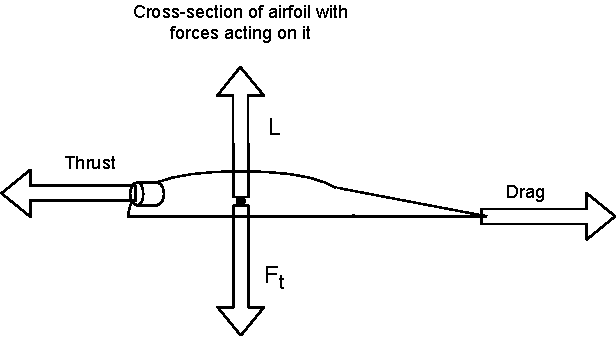
\includegraphics[width=0.7\textwidth]{figures/control_loops/hover_kraftdiagram.pdf}
    \caption{Diagram of the forces acting on each wing in a hover state}
    \label{fig:kraftdiagram}
\end{figure}
The gravitational forces and lift are calculated for the entire drone (eq. \ref{eq:gravity}), while the horizontal forces of thrust and drag are characterized as internal forces acting on each wing and arm of the drone.  
\begin{equation}
\label{eq:gravity}
    F_t = \frac{1}{3}\cdot m_{drone} \cdot g 
\end{equation}
For hover conditions, the lift must be equal to the gravity acting on the drone, necessitated by Newton's second law of motion. \\
The lift, or upwards thrust, is characterized as (\cite{flight_physics}) the lift induced by a conventional tapered airfoil (eq. \ref{eq:lift}). Eq. \ref{eq:rot2speed} is used when converting from angular velocity to velocity.
\begin{align}
    \label{eq:lift}
    L &= \frac{1}{2}*\rho*v^2*A_{wing}*c_L\\
    v &= \omega * r \label{eq:rot2speed}
\end{align}
$\rho$ is the density of the air.
$A_{wing}$ is the surface area of the wing, which has been approximated as shown in fig. \ref{fig:wing_area_approx}.
\begin{figure}[h!]
    \centering
    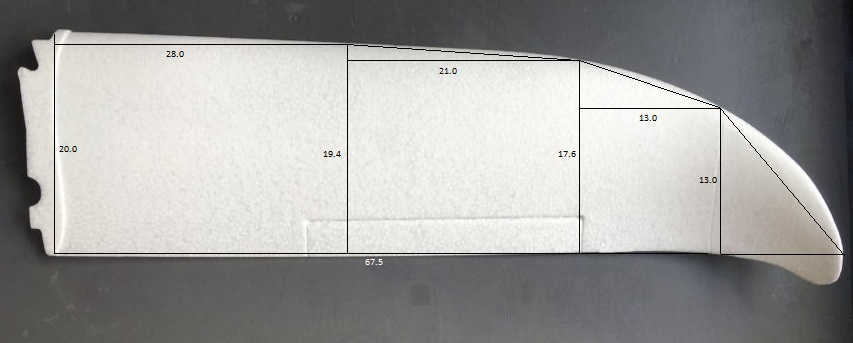
\includegraphics[width=0.9\textwidth]{figures/control_loops/wing_area_approx.jpg}
    \caption{Approximation of wing surface area}
    \label{fig:wing_area_approx}
\end{figure}\\ 
Since the wings are rotating around the center, the wings' speed will be proportionately larger further away from the center. The wings' velocity can be modelled as a function of their rotational velocity, $\omega$ (eq. \ref{eq:rotvel}). 
The average rotational velocity is calculated from "copying" the wing into N wings, each with a velocity corresponding to the inner radius plus its iterational value (ie \textit{i}), or number (eq. \ref{eq:omega_approx}). This is done with a simple for-loop that sums all rotational velocities, $\omega$, and divides with the number of wings, N. For increasingly larger N, this number converges to a slightly better approximation than that of a regular mean over the wing's length. $N=10^6$ was found to be an appropriate size. 
\begin{align}\label{eq:rotvel}
    \omega_i &= \frac{\sqrt{\frac{\frac{2}{3}*m_{drone}*g}{\rho*c_L*A_{wing}}}}{r_{inner}+\frac{i*L_{wing}}{N}}\\
    \omega_{avg} &= \frac{\sum_{i=0}^{N} \omega_i}{N+1}
    \label{eq:omega_approx}
\end{align}
The final variable, $c_L$, is set to a constant value for this calculation.
The lift coefficient, $c_L$, is dependent on the angle of attack (AoA) and can be experimentally calculated. The drag coefficient (denoted $c_D$) and lift coefficient, are calculated with NASA's Foil Sim applet for airfoil approximations. The wing's characteristics can be seen in fig. \ref{fig:liftcoefficient} \cite{lift_coefficient}.

The ratio between lift and drag is also calculated with the applet and can be seen in fig. \ref{fig:LDratio}.

\begin{figure}[h!]
    \centering
    \begin{minipage}[t]{0.48\textwidth}
        \centering
        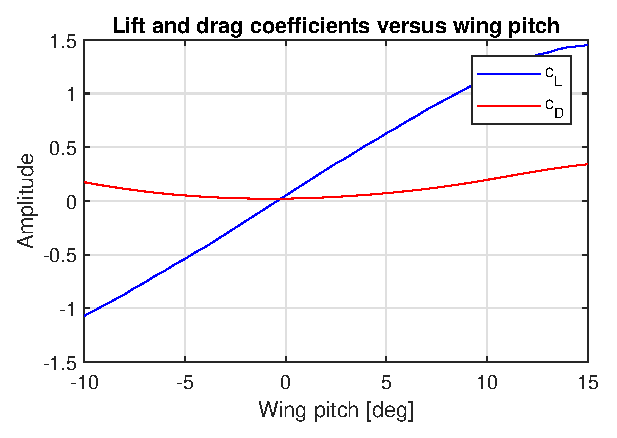
\includegraphics[width=0.96\textwidth]{figures/control_loops/lift_drag_coefficient.eps}
        \caption{The theoretical lift and drag coefficient as a function of the AoA}
        \label{fig:liftcoefficient}
    \end{minipage}%
    \hspace{.03\textwidth}
    \begin{minipage}[t]{0.48\textwidth}
        \centering
        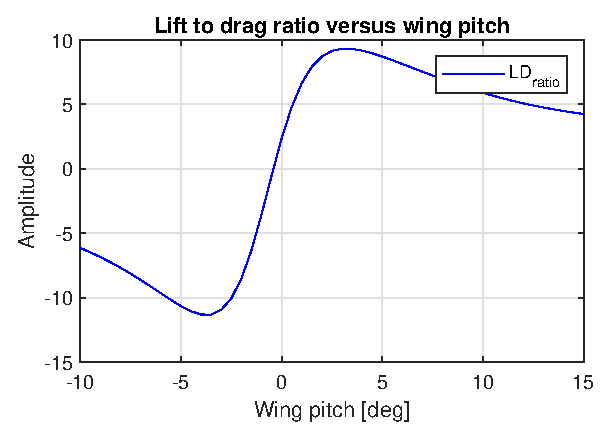
\includegraphics[width=0.96\textwidth]{figures/control_loops/lift_drag_ratio.eps}
        \caption{The theoretical lift-to-drag ratio as a function of AoA}
        \label{fig:LDratio}
    \end{minipage}
\end{figure} 
Although the drone's horizontal axis will be spinning at a constant speed, it is increasingly difficult to calculate and approximate the thrust generated from a propeller motor. Therefore, calculating the motor voltage to lift ratio would require far too many approximations. As such, the results would carry no relevant information to the drone's practical characteristics and, therefore, has not been done. 
Henceforth, the angular velocity will be the measure of the physical model's accuracy.

Varying the lift coefficient, $c_L$, while using the method in eq. \ref{eq:omega_approx}, yields rotational velocities as shown in fig. \ref{fig:liftvariation}

\begin{figure}[h!]
    \centering
    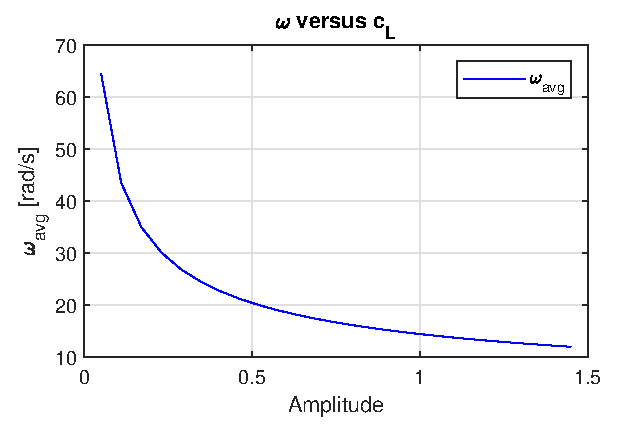
\includegraphics[width=0.5\textwidth]{figures/control_loops/omega_lift_approximation.eps}
    \caption{The average rotational velocity required to hover as a function of the lift coefficient, $c_L$, ($N=10^6$)}
    \label{fig:liftvariation}
\end{figure}

\section{Constraints}
The drone has some physical constraints related to how it was constructed, as it is an atypical drone design. These constraints will have to be considered in the assembly of the control loop.
\begin{itemize}
\label{list:constraints}
    \item The motors are wired in such a way that they are only provided positive voltages. Consequently, they will only be able to spin clockwise (spinning the drone counter-clockwise), thereby creating thrust in their positive z-direction (one-way horizontal rotation).
    \item The wing pitch is very restricted in articulation, as seen in fig. \ref{fig:liftcoefficient}. Any AoA out of this range will most likely cause stalling.
\end{itemize}

\section{System controller}
In this section, design of the system controller will be examined. To be able to control the angular velocity, the drone's physical properties from motor voltage to rotation need to be determined. This means deriving the natural transfer function, which can be found from the step response of the system. 
The finished control system consists of one controller, that will regulate the drone's angular velocity around its z-axis based on a set reference point. \\
The controller will output voltages that adjust the propeller motors to maintain a steady velocity.

\subsection{Natural transfer function of the system}
In this section, it is discussed how a natural transfer function for the system can be derived. The drone will receive a step in voltage, when it's in a steady state rotation, where the output angular velocity will be analyzed both manually and correlated with the assistance of Matlab's Systems Identification Toolbox \cite{SysidToolbox}. This step will be conducted both on- and off-ground.\\

\textbf{Deriving a transfer function:}\\ \label{tf_teori}Manually deriving a transfer function from an open-loop step response can realistically only be done for a very simple system with one or two poles in the same location. For the 2nd order system with coinciding poles, the damping ratio is unity. This is also known as the over-dampened case. Here, the poles are real and negative.
To find this pole, the time constant, $\tau$, must be found. $\tau$ is located as the point in time when the output has reached 63.2\% of its final value. The pole is then found as the negative inverse of $\tau$ \cite{reguleringsbog}. For a 1st order system of the following form, $h(s) = \frac{b}{s+a}$, the static gain is found as $\frac{b}{a}$. From this expression, \textit{b} can be isolated. 

Otherwise, to determine a transfer function for a system, a tool like System Identification Toolbox is useful \cite{SysidToolbox}. It uses a nonlinear least-squares algorithm to fit a user-specified number of poles and zeros to the given data. The data is a step starting from 0, both with input values and output values. It returns a fitted transfer function and a percentage of how good the fit is. 

When analysing the results, a 1st order transfer function will be derived manually once. Thereafter, System Identification Toolbox will be used instead. 

\subsection{Controller type}
As previously mentioned, the drone has physical constraints, therefore the implemented controller will need to have an insignificant overshoot. A differential controller of the right proportions will ensure the right amount of damping and that the overshoot is minimal or non-existent. \\
To ensure minimal steady-state error along with system stability and a fast-enough response, a proportional gain is a natural addition to the differential part. However, the proportional gain is restricted to small values due to the physical constraints of the prop motors' input voltage range. \\
Furthermore, in the process of keeping the controller's response precise and relevant, a simple feed-forward element will be implemented to account for any significant discrepancies. The feed-forward branch works to complement the feedback PD-controller, as it maintains a rather fast overall response of the system. \\
The block diagram is in fig. \ref{fig:controlblock}.

\begin{figure}[h!]
    \centering
    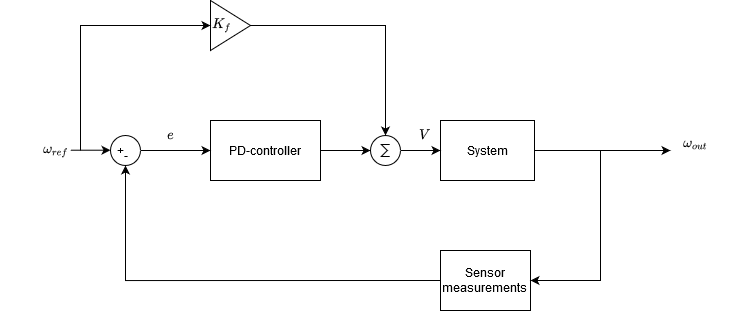
\includegraphics[width=1.0\textwidth]{figures/control_loops/control_block_diagram.png}
    \caption{Block diagram of PD control loop with a feed-forward branch}
    \label{fig:controlblock}
\end{figure}

The values of $K_P$ and $K_D$ will be determined from the system transfer function. The feed-forward gain, $K_f$ will be found by approximating the linear relationship between motor voltage and angular velocity. From this, an expression will be derived. It will act as a system "predictor". \\
For the system, the feed-forward will act as a coarse adjuster, while the PD-controller will act as a fine-tuner.\\
The final closed-loop transfer function becomes (with system named $A(s)$):
\begin{equation}
    G(s) = \frac{\omega_{out}(s)}{\omega_{ref}(s)} = \frac{A(s)*\left(PD(s)+K_f\right)}{1+A(s)*PD(s)}
\end{equation}


\section{Chapter summary}
This chapter introduced the physics of the drone in a hover state. An approximation of the wings' properties was derived, and a controller to regulate the drone's angular velocity was proposed. Additionally its block diagram as well as transfer function were examined. Finally, ways of determining a transfer function from a step response was elaborated upon.\\
The groundwork for a well-functioning control loop has been made. Derivation and implementation of transfer functions and control loop, as well as performance evaluation will be completed in section \ref{results:rotcontroller}.  
